\begin{frame}{About me}
	\framesubtitle{
		\url{https://pierrebeaujean.net/}}
	\begin{itemize}
		\item 2006: Ubuntu 6.06 LTS, from a friend
		\item 2007: Started learning programming from the \textit{Site du Zéro} (now deceased!).
		\item 2009: chose to study chemistry instead, but keeps Linux
		\item 2015: Switching to \textit{Zeste de Savoir} (I'm still there!)
		\item January 2015: Started and fulfilled a master’s thesis in Quantum Chemistry
		\item September 2015: started (and recently fulfilled!) a PhD in Quantum Chemistry, as Teaching Assistant
		\item September 2017: started (and fulfilled) a bachelor in computer science (evening classes)
		\item September 2021: started to work for the Belgian NCC for HPC.
	\end{itemize}
	
\end{frame}

\begin{frame}{Preliminary notes}
	\begin{itemize}
		\item Jokes and opinions are my own, not the one of the NCC Belgium ;)
		\item First of all, ``Premature optimization is the root of all evil'' (Sir Tony Hoare). And code optimization is an art, and the result depends on the target architecture (cache size, instruction set, connectivity, etc. See \cdx{lscpu}).
		\item Here, we will not look for the best optimized code. We will just look at the effect of some modifications (and sometimes, the assembler).
		\item Codes are in C (but could be in Fortran), compiled with \cdx{gcc} (Intel compiler may provide better results on Intel architectures). 
		\item Two simple examples from linear algebra (LAPACK): \cdx{*dot} and \cdx{*axpy}. If you ever need that, use libraries instead!
	\end{itemize}
\begin{center}
	
\includegraphics[width=.25\textwidth]{qrcode}\\
	\url{https://github.com/pierre-24/HPC-parallel-introduction}
\end{center}
\end{frame}

\begin{frame}[fragile]{The examples for today}
	\begin{itemize}
		\item \cdx{(s|d)dot}: dot product of two vectors: $r = \vec{x}\cdot\vec{y}$.
		\begin{ccode}
float sdot(int n, float* x, float* y) {
	float sum = .0f;
	if (n > 0) {
		for(int i=0; i < n; i++)
			sum += y[i] * x[i];
	}
	return accum;
}
		\end{ccode}
	Note: actually use a \textbf{Kahan sum}!
		\item \cdx{(s|d)axpy}: generalized vector addition: $\vec y = \vec y + a\,\vec x$.
		\begin{ccode}
void saxpy(int n, float alpha, float* x, float* y) {
	if (n > 0 && alpha != 0.f) {
		for(int i=0; i < n; i++)
			y[i] += alpha * x[i];
	}
}
		\end{ccode}
	\end{itemize}
\end{frame}

\begin{frame}[fragile]{Preamble: Kahan sum}
	\url{https://en.wikipedia.org/wiki/Kahan_summation_algorithm}
	\begin{columns}
	\column[t]{.65\textwidth}
	\begin{ccode}
float sdot(int n, float* x, float* y) {
	float sum = .0f, c = .0f;
	float addend, tmpSum;
	if (n > 0) {
		for(int i=0; i < n; i++) {
			addend = y[i] * x[i] - c;
			tmpSum = sum + addend;
			c = (tmpSum - sum) - addend;
			sum = tmpSum;
		}
	}
	return sum;
}
	\end{ccode}
\column[t]{.35\textwidth}
	\begin{center}
		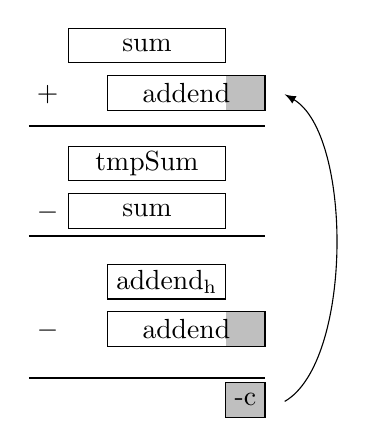
\begin{tikzpicture}
			\draw (0,0) rectangle +(2,1.25em) node[midway]{\cdx{sum}};
			\fill[black!25] (2,-.6) rectangle +(.5,1.25em);
			\draw (.5,-.6) rectangle +(2,1.25em) node[midway]{\cdx{addend}};
			\draw (0,-.4)  node[left]{$+$};
			\draw[thick] (-.5,-.8) -- +(3,0);
			\draw (0,-1.5) rectangle +(2,1.25em) node[midway]{\cdx{tmpSum}};
			\draw (0,-2.1) rectangle +(2,1.25em) node[midway]{\cdx{sum}};
			\draw (0,-1.9)  node[left]{$-$};
			\draw[thick] (-.5,-2.2) -- +(3,0);
			\draw (.5,-3) rectangle +(1.5,1.25em) node[midway]{\cdx{addend}\textsubscript{h}};
			\fill[black!25] (2,-3.6) rectangle +(.5,1.25em);
			\draw (.5,-3.6) rectangle +(2,1.25em) node[midway]{\cdx{addend}};
			\draw (0,-3.4)  node[left]{$-$};
			\draw[thick] (-.5,-4) -- +(3,0);
			\draw[fill=black!25] (2,-4.5) rectangle +(.5,1.25em) node[midway]{-\cdx{c}};
			\draw[-latex] (2.75,-4.3) .. controls +(30:1) and +(-30:1) .. (2.75,-.4);
		\end{tikzpicture}
	\end{center}
\end{columns}
\end{frame}

\begin{frame}{Preamble: don't forget 'bout optimization}
	\begin{table}
		\begin{tabular}{l cc c cc}
			\toprule
			& \multicolumn{2}{c}{\cdx{*dot}} &&\multicolumn{2}{c}{\cdx{*axpy}}\\
			& \cdx{s} & \cdx{d} && \cdx{s} & \cdx{d}\\
			\midrule
			\cdx{-O0} & 426.5 & 420.4 && 137.3 & 136.4\\
			\cdx{-O1} & 141.1 & 140.1  && 30.7 & 31.7\\
			\bottomrule
		\end{tabular}
		\caption{Average running times (in ms) with \cdx{-N 1000}, on $2^{24}$ numbers.}
	\end{table}
	\begin{itemize}
		\item Ran on AMD EPYC 7542, and compiled with GCC 10.2
		\item Compilers does a decent job at optimizing (see \url{https://gcc.gnu.org/onlinedocs/gcc/Optimize-Options.html} for the details)
		\item \cdx{-O2} and \cdx{-O3} include stuff we will see later on (but you \textbf{should} use \cdx{-O3}, or even \cdx{-Ofast}).
		\item If you are brave enough \cdx{objdump -dS -M intel <program, compiled with -g>}.
	\end{itemize}
\end{frame}